\begin{figure}
    \begin{center}
    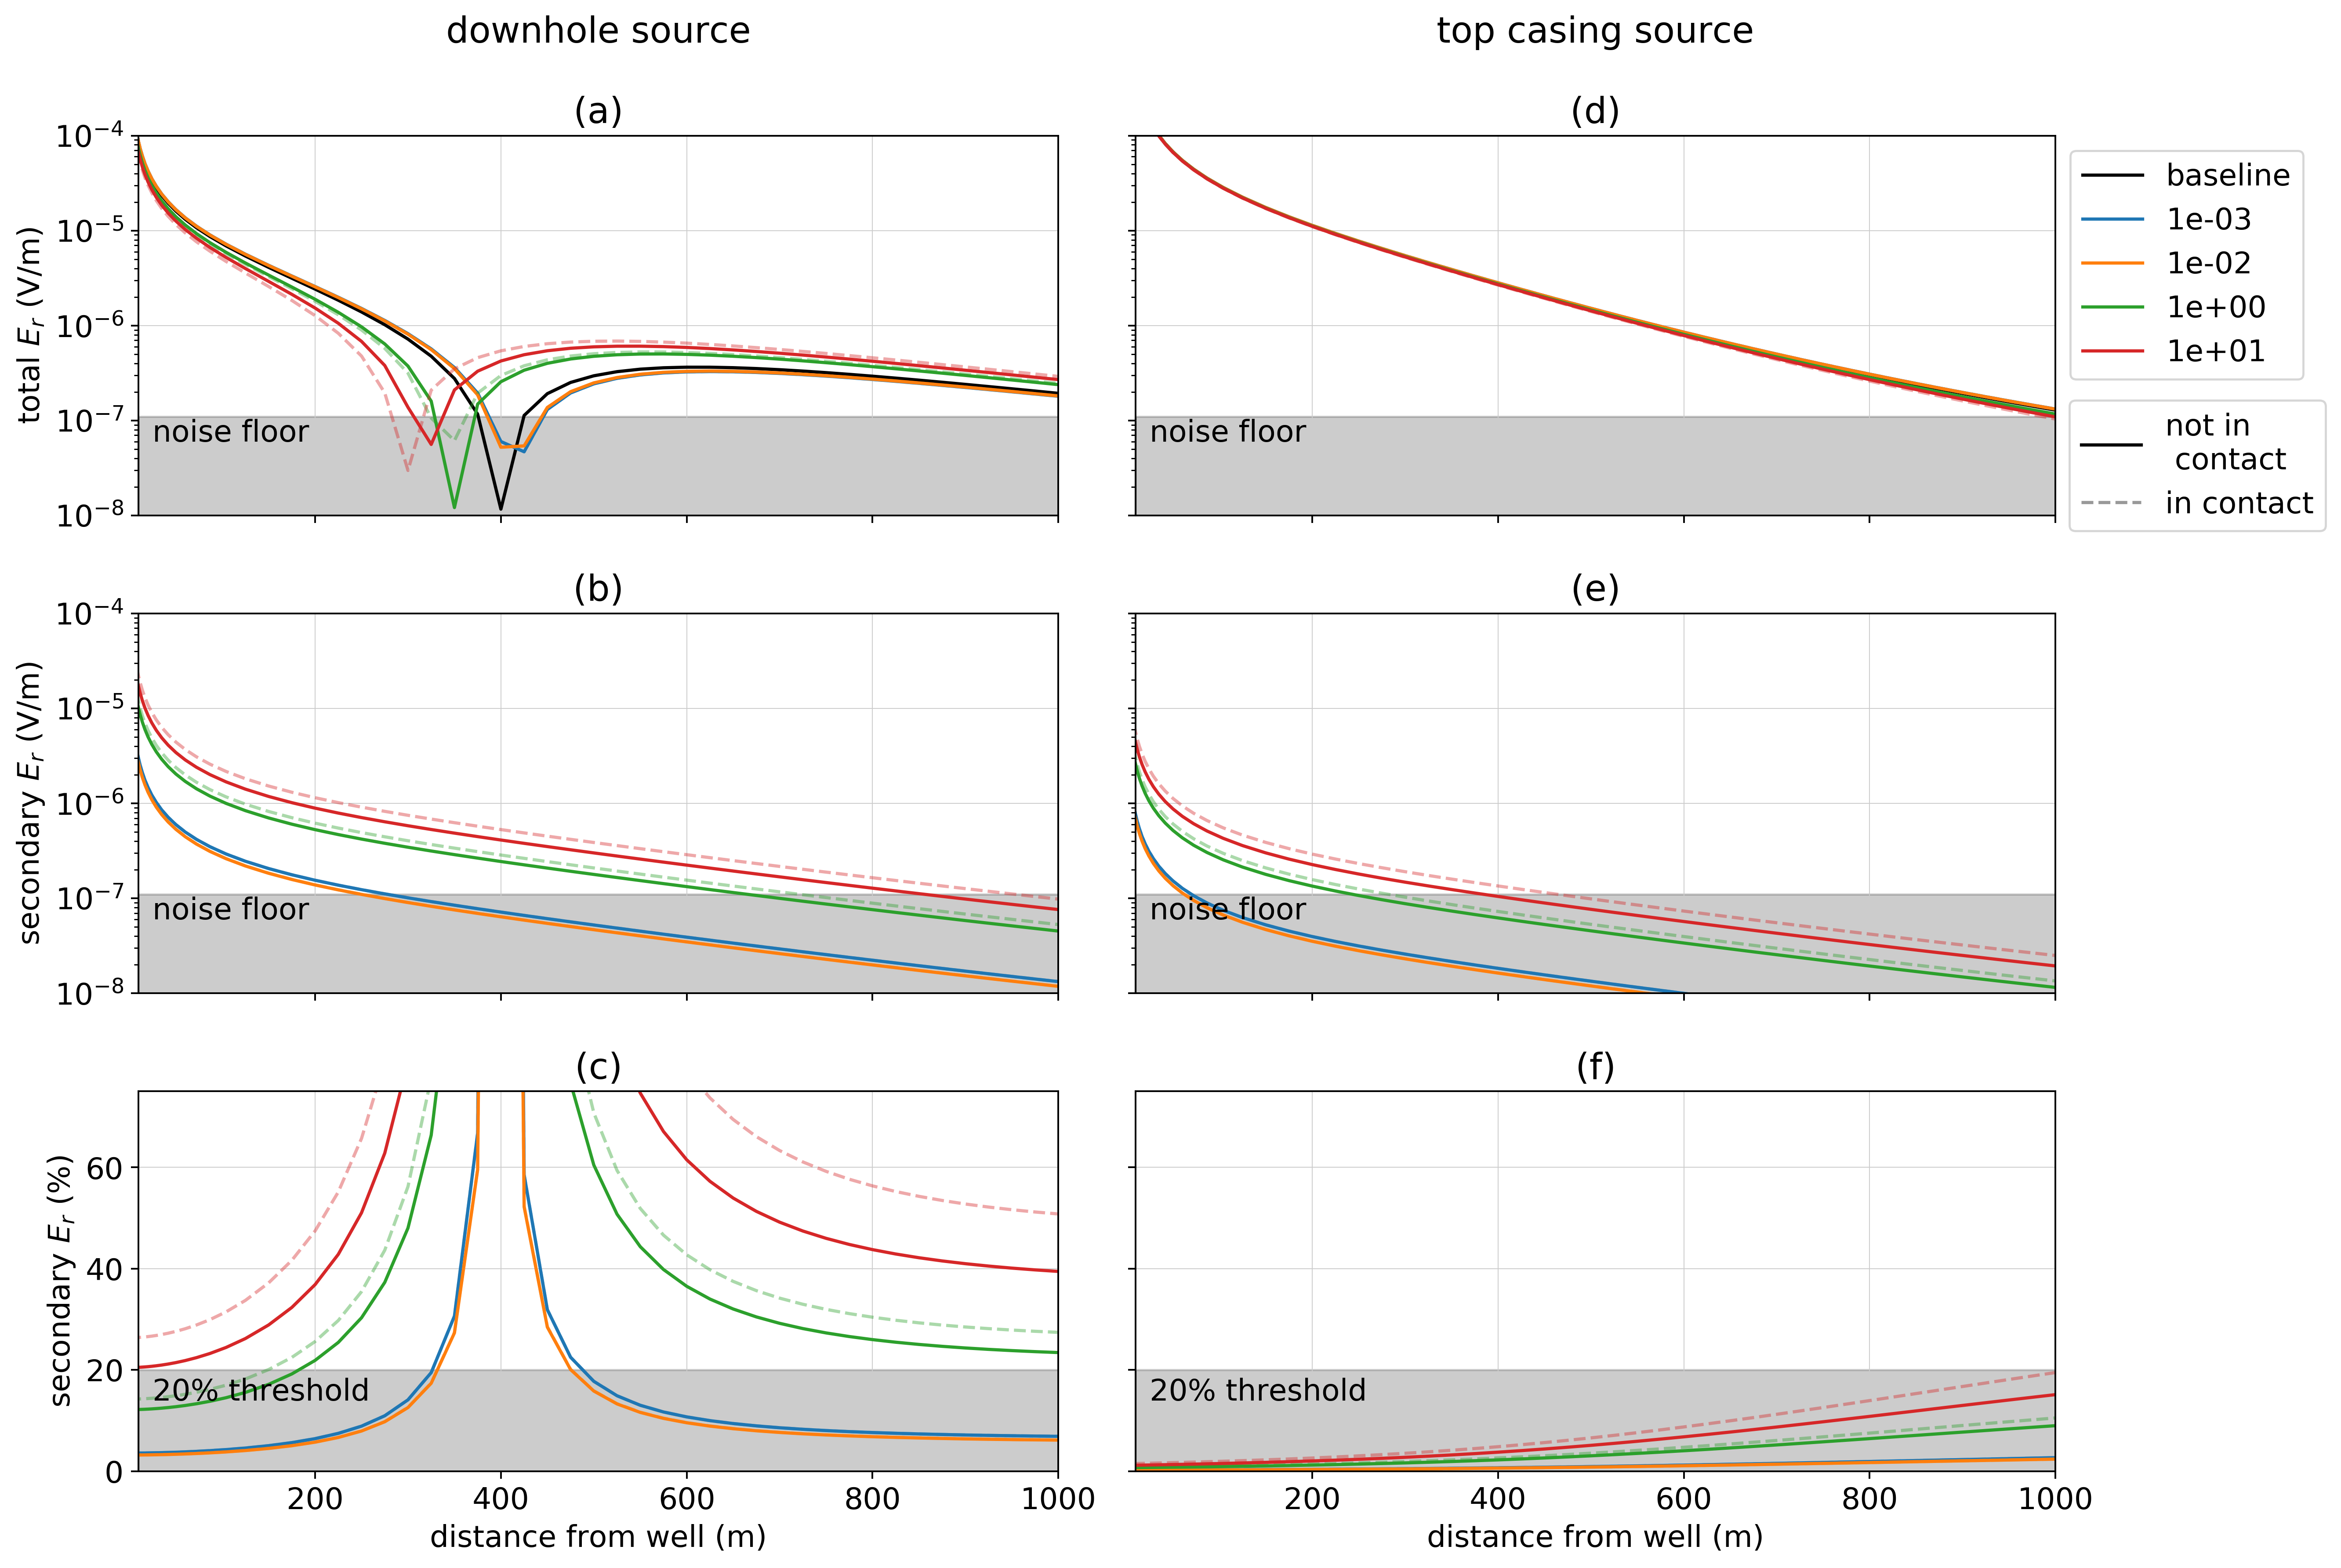
\includegraphics[width=\textwidth]{figures/offset_electric_fields.png}
    \end{center}
\caption{
    Radial electric field at the surface as the conductivity of a cylindrical target, which is not contact with the well,
    is varied. The target has a radius of 25m and extends in depth from 900m to 925m. The return electrode
    is on the surface, 500m from the well and data are measured along a line perpendicular to the source.
    The panels on the left show
    (a) the total electric field, (b) the secondary electric field with respect to a primary that does not include the target,
    and (c) the secondary electric field as a percentage of the primary for a survey in which the positive electrode is
    positioned downhole at 912.5m depth. The panels on the right similarly show (d) the total electric field, (e) the
    secondary electric field, and (f) the secondary electric field as a percentage of the primary for a top-casing experiment.
    The data shown in Figure \ref{fig:target_electric_fields}, for the target in contact with the well,
    are plotted in the dashed, semi-transparent lines for reference.
}
\label{fig:offset_electric_fields}
\end{figure}
